\begin{figure}
\centering
\fbox{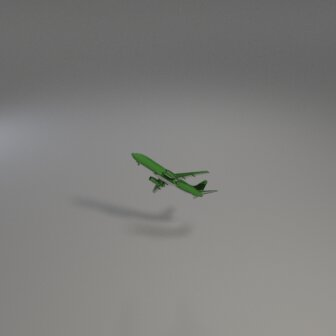
\includegraphics[width=0.4\linewidth]{figures/samples/so3.jpg}}
\begin{minted}[breaklines]{python}
add(shape='airliner', size='tiny', color='green', material='matte', rotation=(-0.798, 0.124, 0.590, -0.562, -0.507, -0.654))
\end{minted}
\caption{\textbf{SO(3) Range-Gap Train Sample.} (\cref{sssec:so3})}
\label{fig:code_so3}
\end{figure}